\documentclass[a4paper,11pt,UTF8]{article}
\usepackage{ctex}
\usepackage{amsmath,amsthm,amssymb,amsfonts}
\usepackage{amsmath}
\usepackage[a4paper]{geometry}
\usepackage{graphicx}
\usepackage{microtype}
\usepackage{siunitx}
\usepackage{booktabs}
\usepackage[colorlinks=false, pdfborder={0 0 0}]{hyperref}
\usepackage{cleveref}
\usepackage{esint} 
\usepackage{graphicx}
\usepackage{ragged2e}
\usepackage{pifont}
\usepackage{extarrows}
\usepackage{mathptmx}
\usepackage{float}
\usepackage{caption}
\usepackage{graphicx} %插入图片的宏包
\usepackage{float} %设置图片浮动位置的宏包
\usepackage{subfigure} %插入多图时用子图显示的宏包
\renewcommand{\thesubfigure}{(\roman{subfigure})}%此外,还可设置图编号显示格式,加括号或者不加括号
\captionsetup[figure]{name={Figure}}
%opening
\title{Microelectronics Circuit Analysis and Design Homework(3rd)}
\author{Yuejin Xie \quad U202210333}
\date{Sept 15th, 2023 }
\begin{document}
\maketitle
\noindent1.45 The diode cut-in voltage is $V_\gamma = 0.7$ V for the circuits shown in Figure
P1.45. Plot $V_O$ and $I_D$ versus $I_I$ over the range $0 \leq I_I \leq 2 $mA for the circuit
shown in (a) Figure P1.45(a), (b) Figure P1.45(b), and (c) Figure
P1.45(c).\\
\begin{figure}[H]
	\centering  %图片全局居中
	\subfigure[a]{
		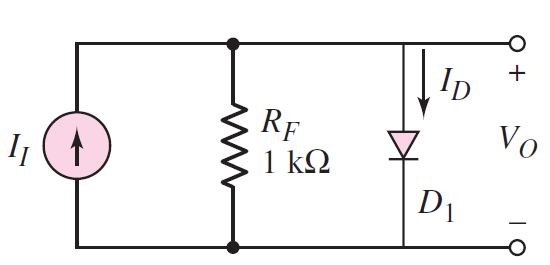
\includegraphics[scale=0.2]{MD1_45a.png}}
	\subfigure[b]{
		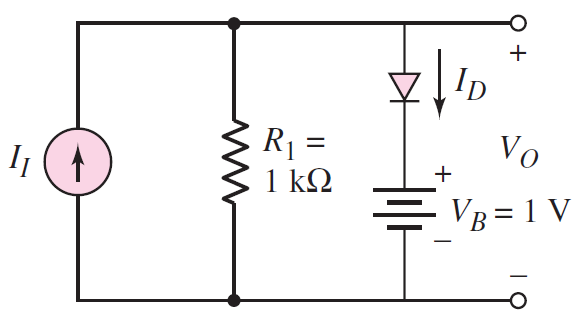
\includegraphics[scale=0.2]{MD1_45b.png}}
	\subfigure[c]{
		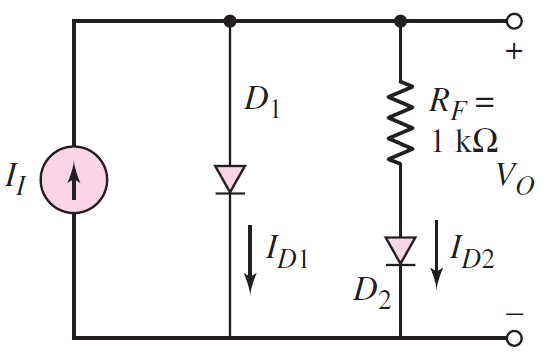
\includegraphics[scale=0.2]{MD1_45c.png}}
	\caption{(a)}
\end{figure}
\noindent Solution:\\
(a)KCL:$\displaystyle I_I=\frac{V_O}{R_F}+I_D$\\
When $V_O\geq V_\gamma=0.7$V, the diode is conducted, so $R_F$ is shorted $\Rightarrow I_D= I_I-0.7, V_O=0.7$V\\
To satisfy the circumstance, we need $I_I\geq0.7$mA.\\
When $V_O\leq V_\gamma=0.7$V, the diode isn't conducted and can be regarded as open$\Rightarrow I_D= 0, V_O=I_IR_F$\\
To satisfy the circumstance, we need $I_I\leq0.7$mA.\\
\begin{figure}[H]
	\centering  %图片全局居中
	\subfigure[$V_O-I_I$]{
		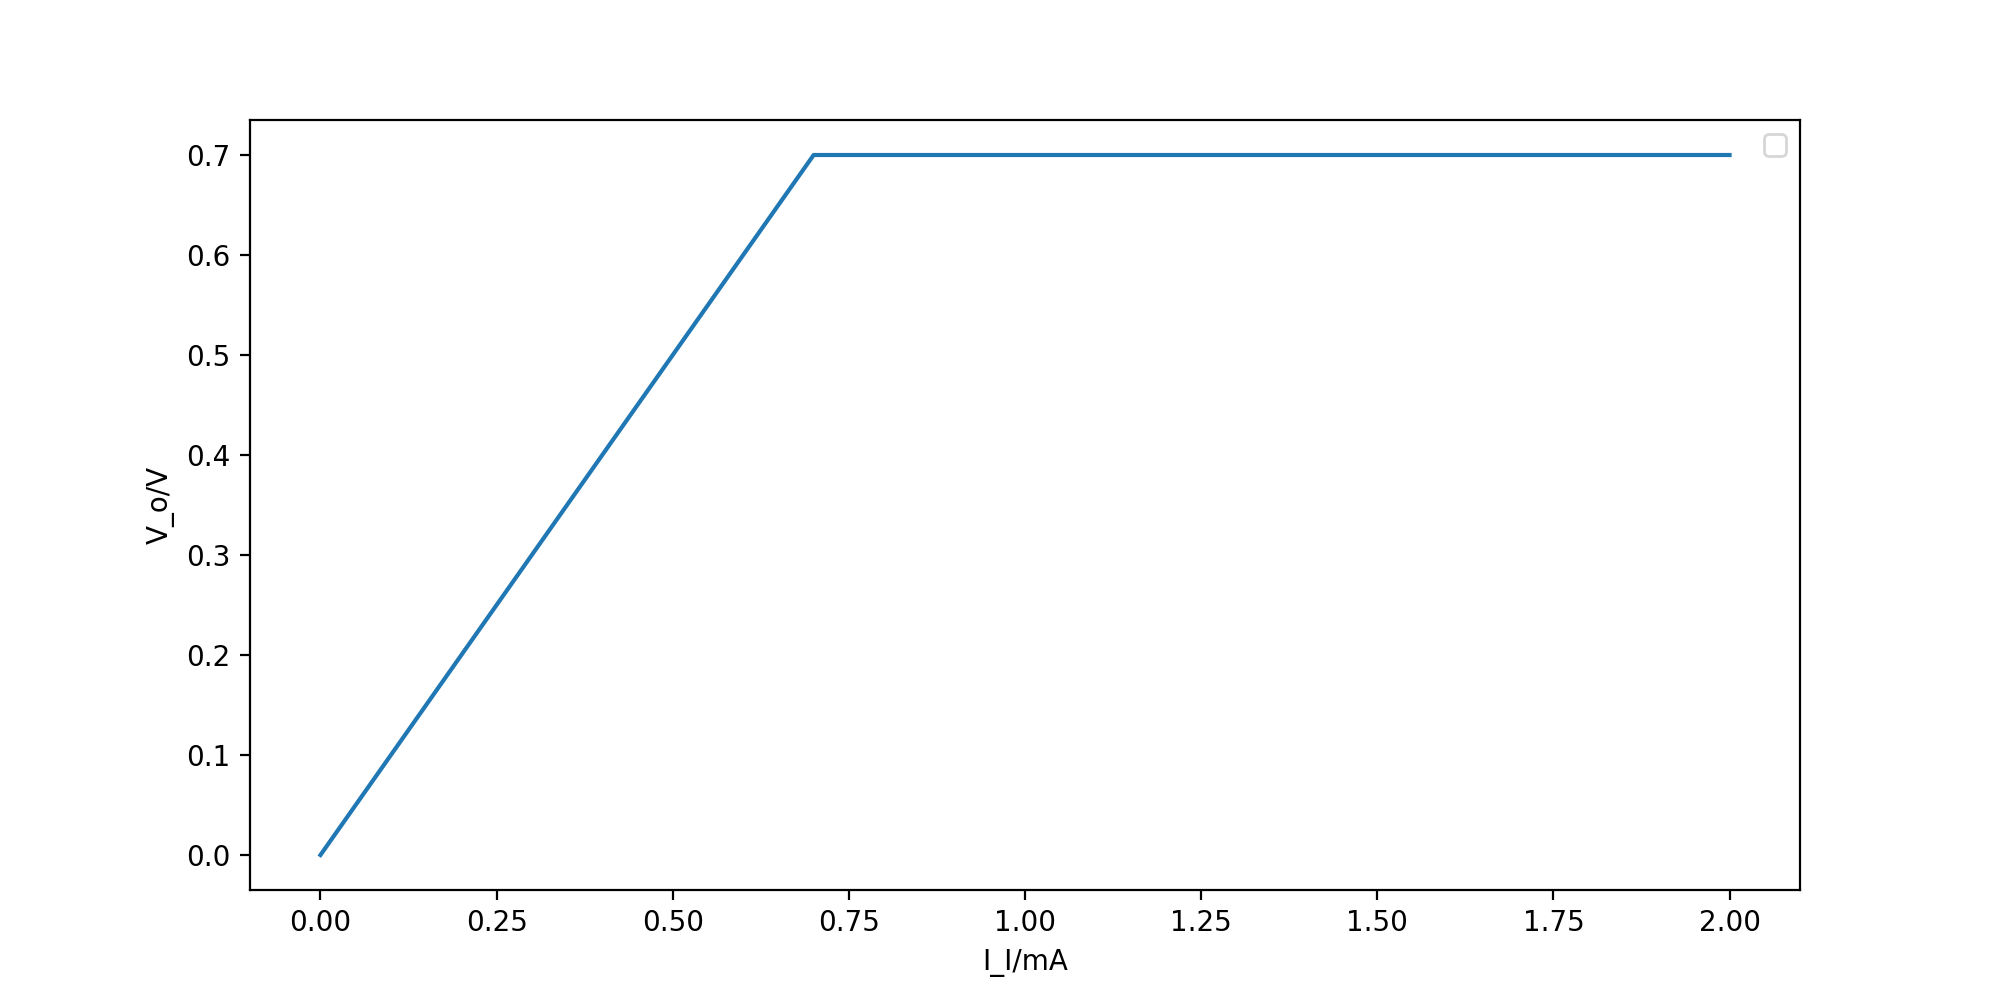
\includegraphics[scale=0.27]{MD1.45_1.png}}
	\subfigure[$I_D-I_I$]{
		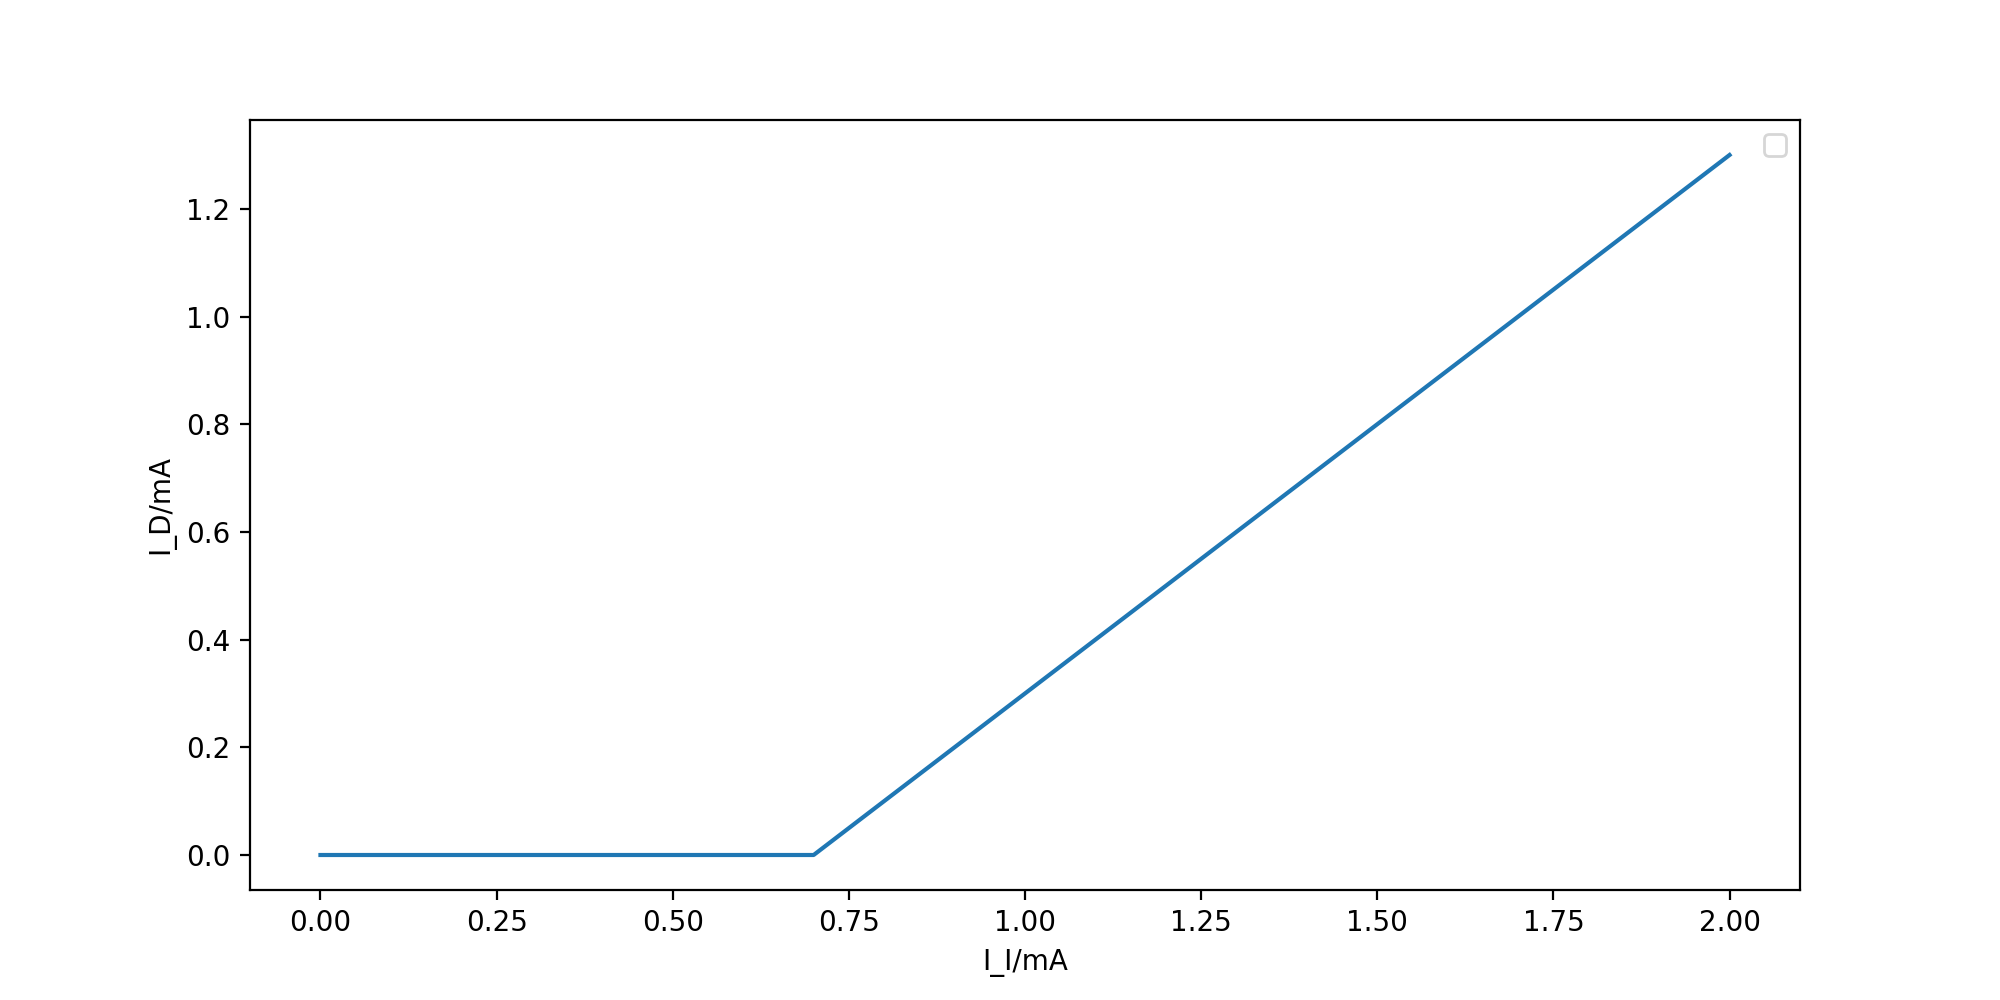
\includegraphics[scale=0.27]{MD1.45_2.png}}
	\caption{(a)}
\end{figure}
\noindent(b)KCL:$\displaystyle I_I=\frac{V_O}{R_F}+I_D$\\
When $V_O\geq V_\gamma+V_B=1.7$V, the diode is conducted, so $R_F$ is shorted $\Rightarrow I_D= I_I-1.7, V_O=1.7$V\\
To satisfy the circumstance, we need $I_I\geq1.7$mA.\\
When $V_O\leq V_\gamma+V_B=1.7$V, the diode isn't conducted and can be regarded as open$\Rightarrow I_D= 0, V_O=I_IR_F$\\
To satisfy the circumstance, we need $I_I\leq1.7$mA.\\
\begin{figure}[H]
	\centering  %图片全局居中
	\subfigure[$V_O-I_I$]{
		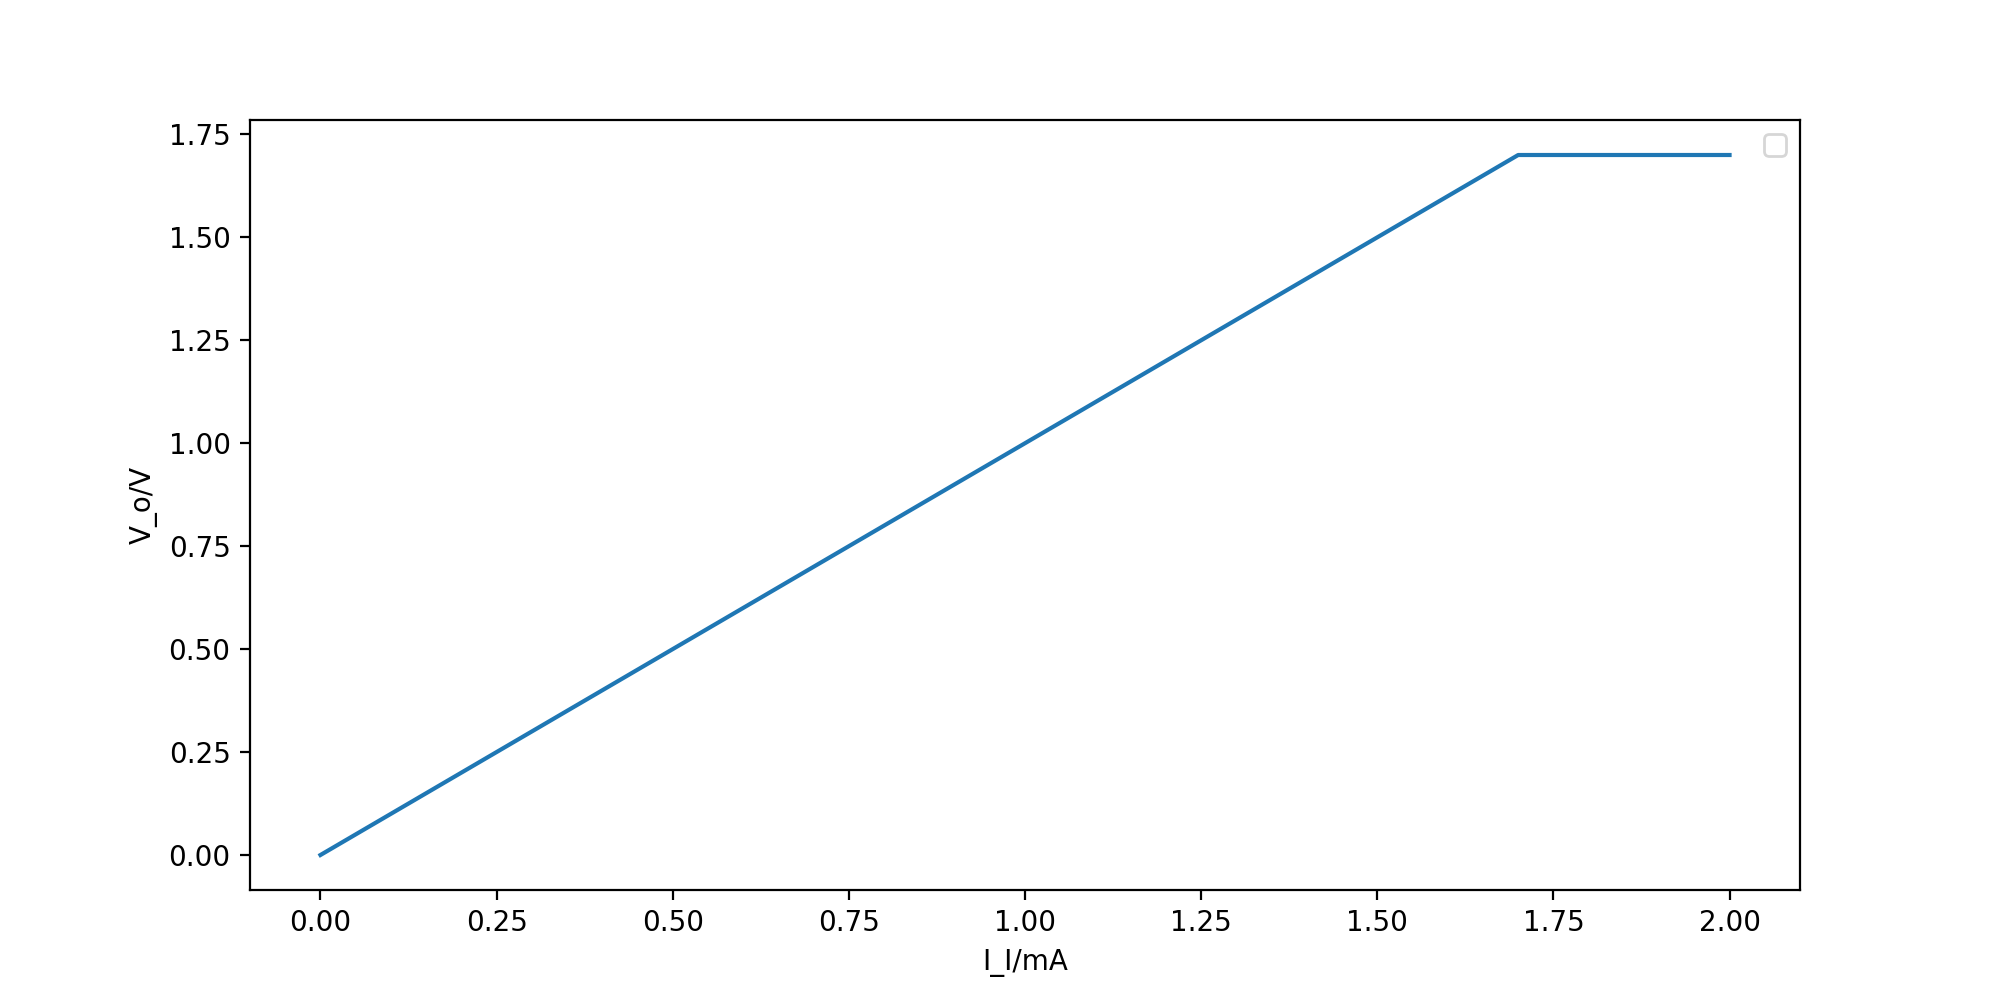
\includegraphics[scale=0.27]{MD1.45_3.png}}
	\subfigure[$I_D-I_I$]{
		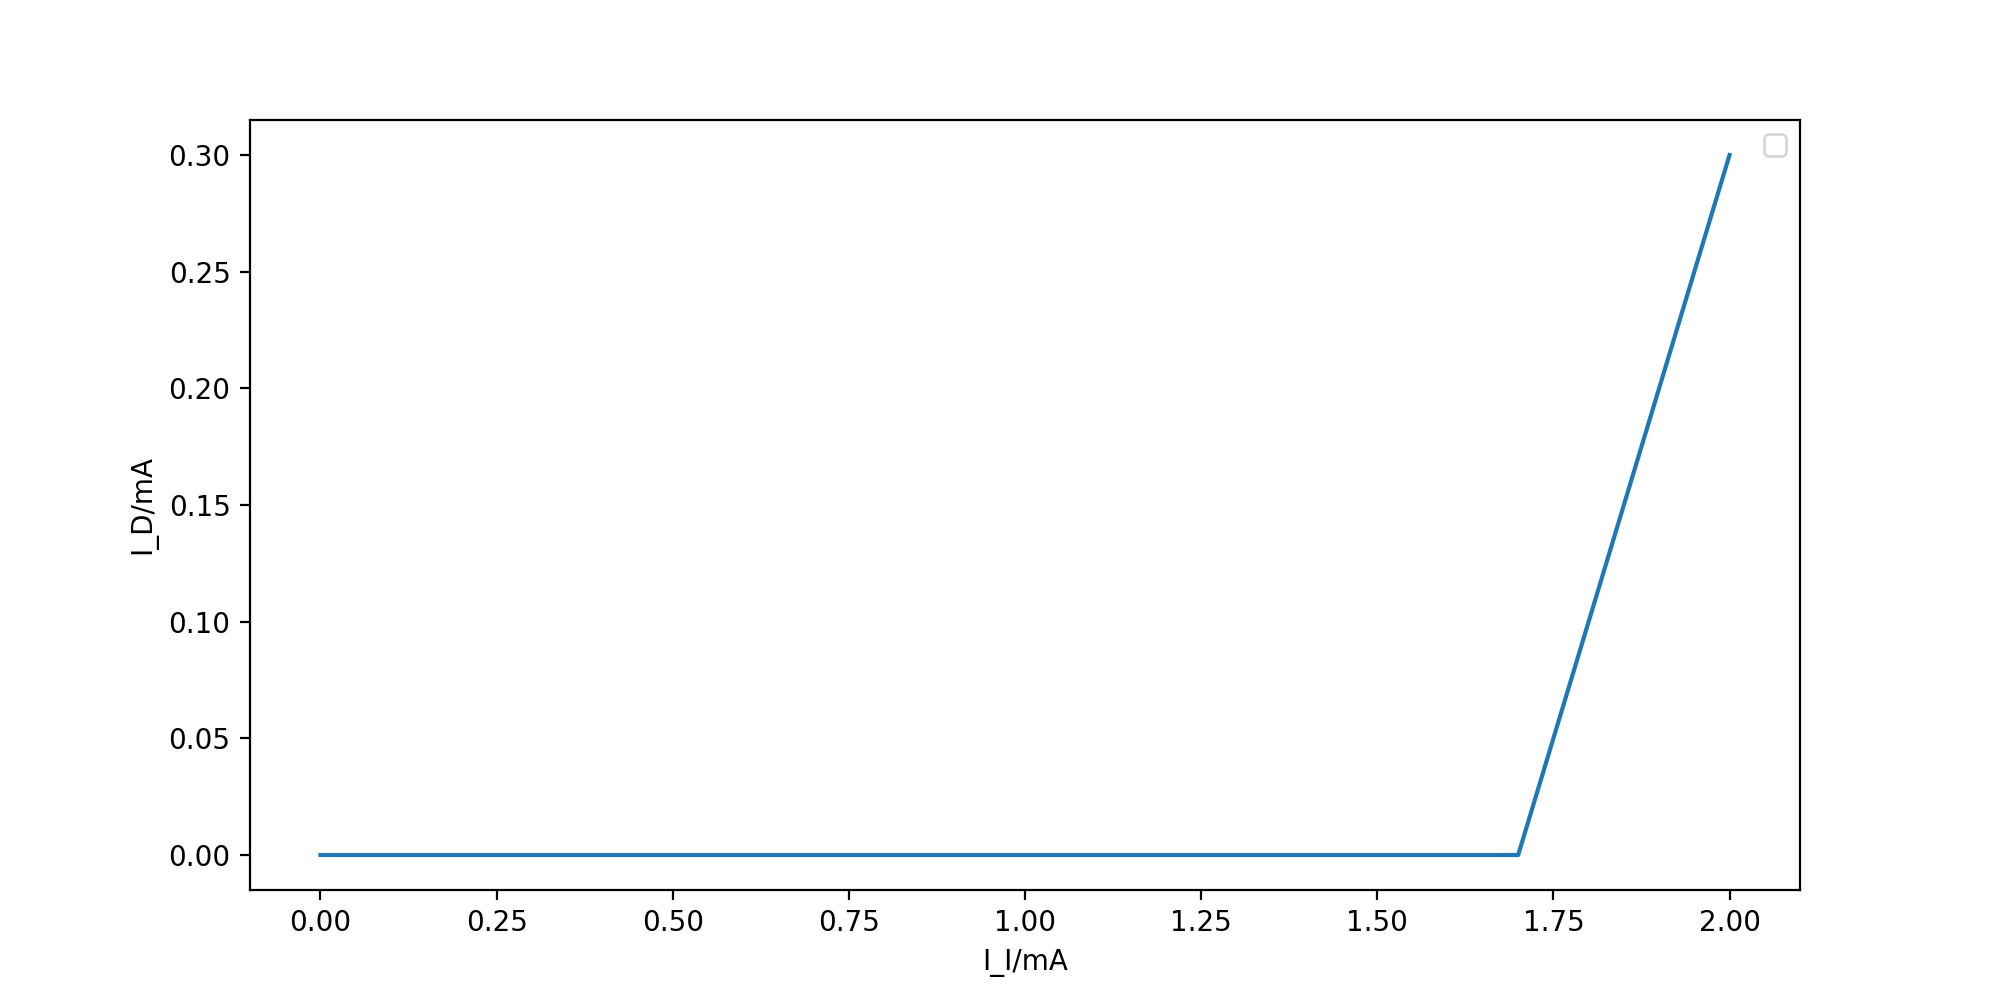
\includegraphics[scale=0.27]{MD1.45_4.png}}
	\caption{(b)}
\end{figure}
\noindent(c)
We can know that $D_1$ will be conducted forever(ideal Current Source), and at this time $D_2 \text{and} R_F$ will be shorted.\\
$\Rightarrow V_O = 0.7 V, I_{D1} = I_I \text{ and } I_{D2} = 0$\\
\begin{figure}[H]
	\centering  %图片全局居中
	\subfigure[$V_O-I_I$]{
		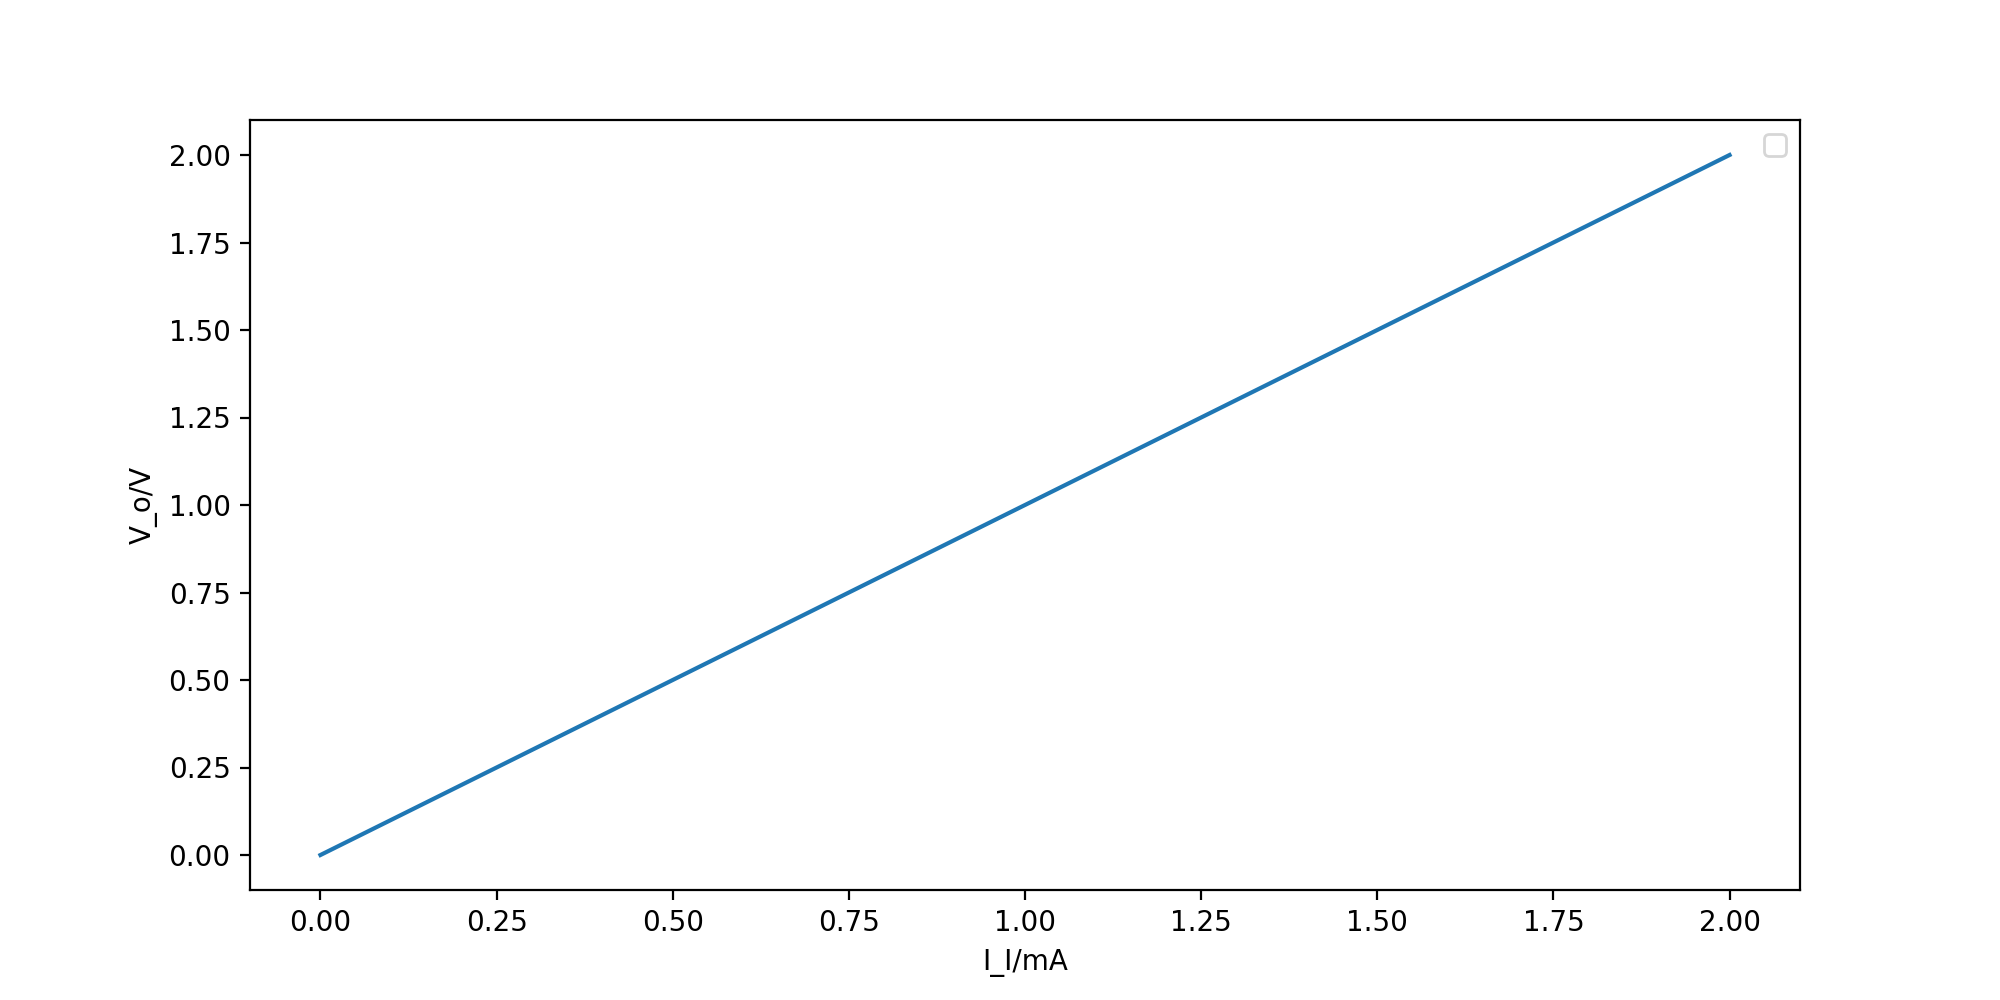
\includegraphics[scale=0.5]{MD1.45_5.png}}\\
	\subfigure[$I_{D1}-I_I$]{
		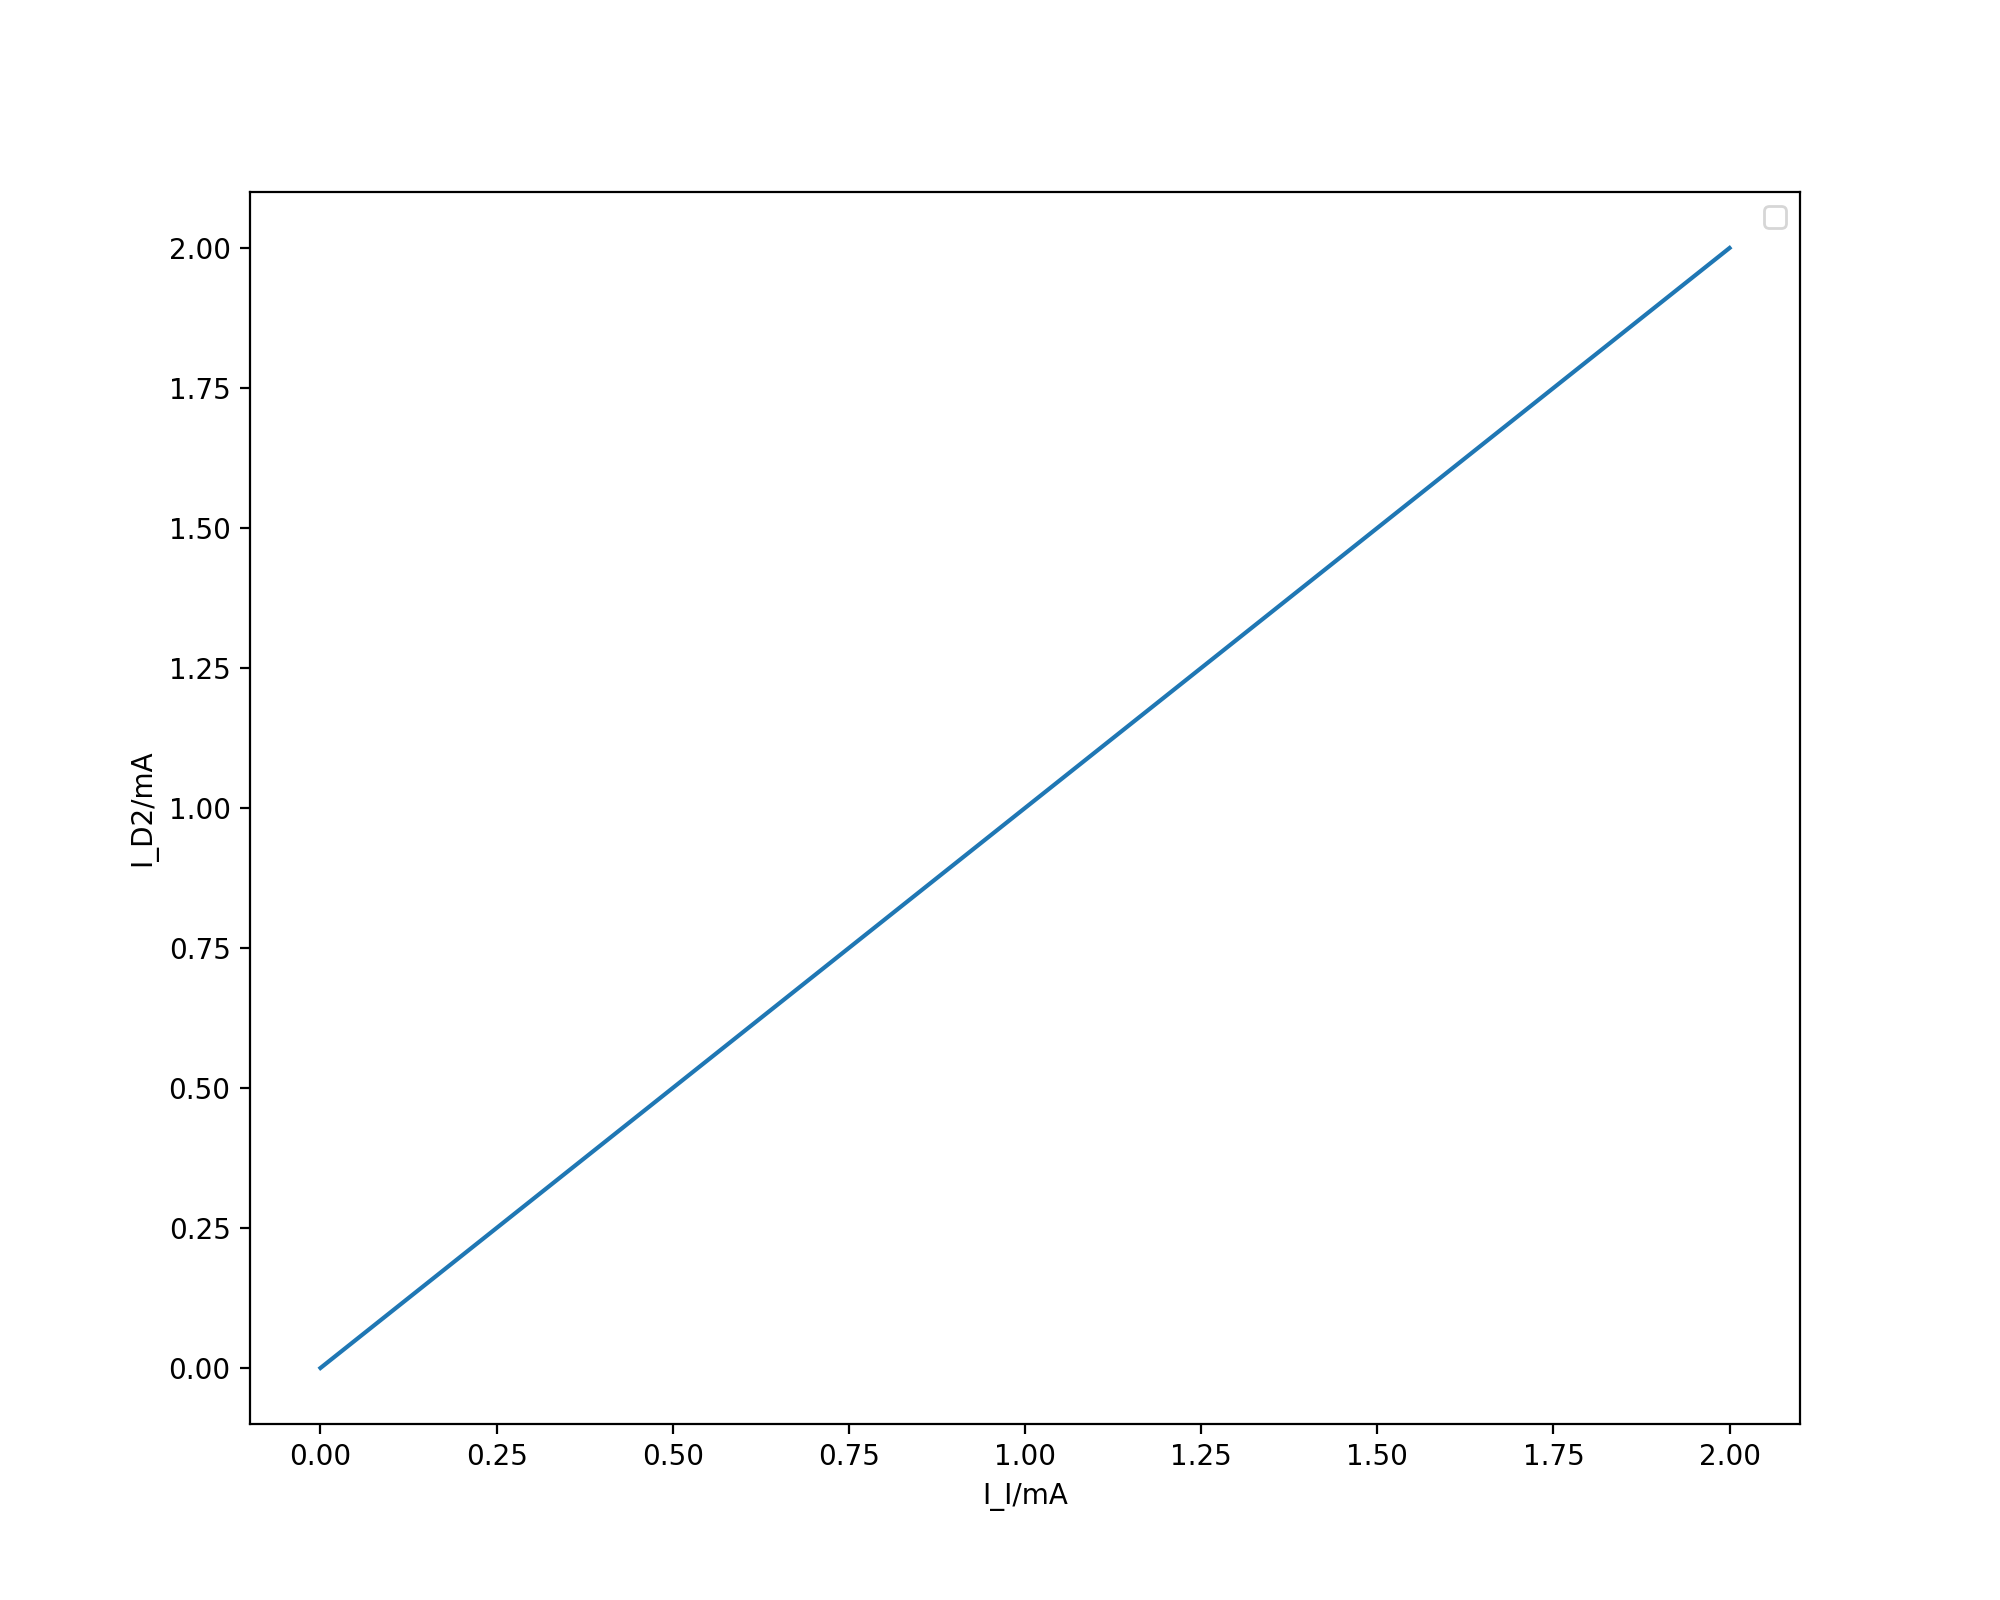
\includegraphics[scale=0.28]{MD1.45_6.png}}
	\subfigure[$I_{D2}-I_I$]{
		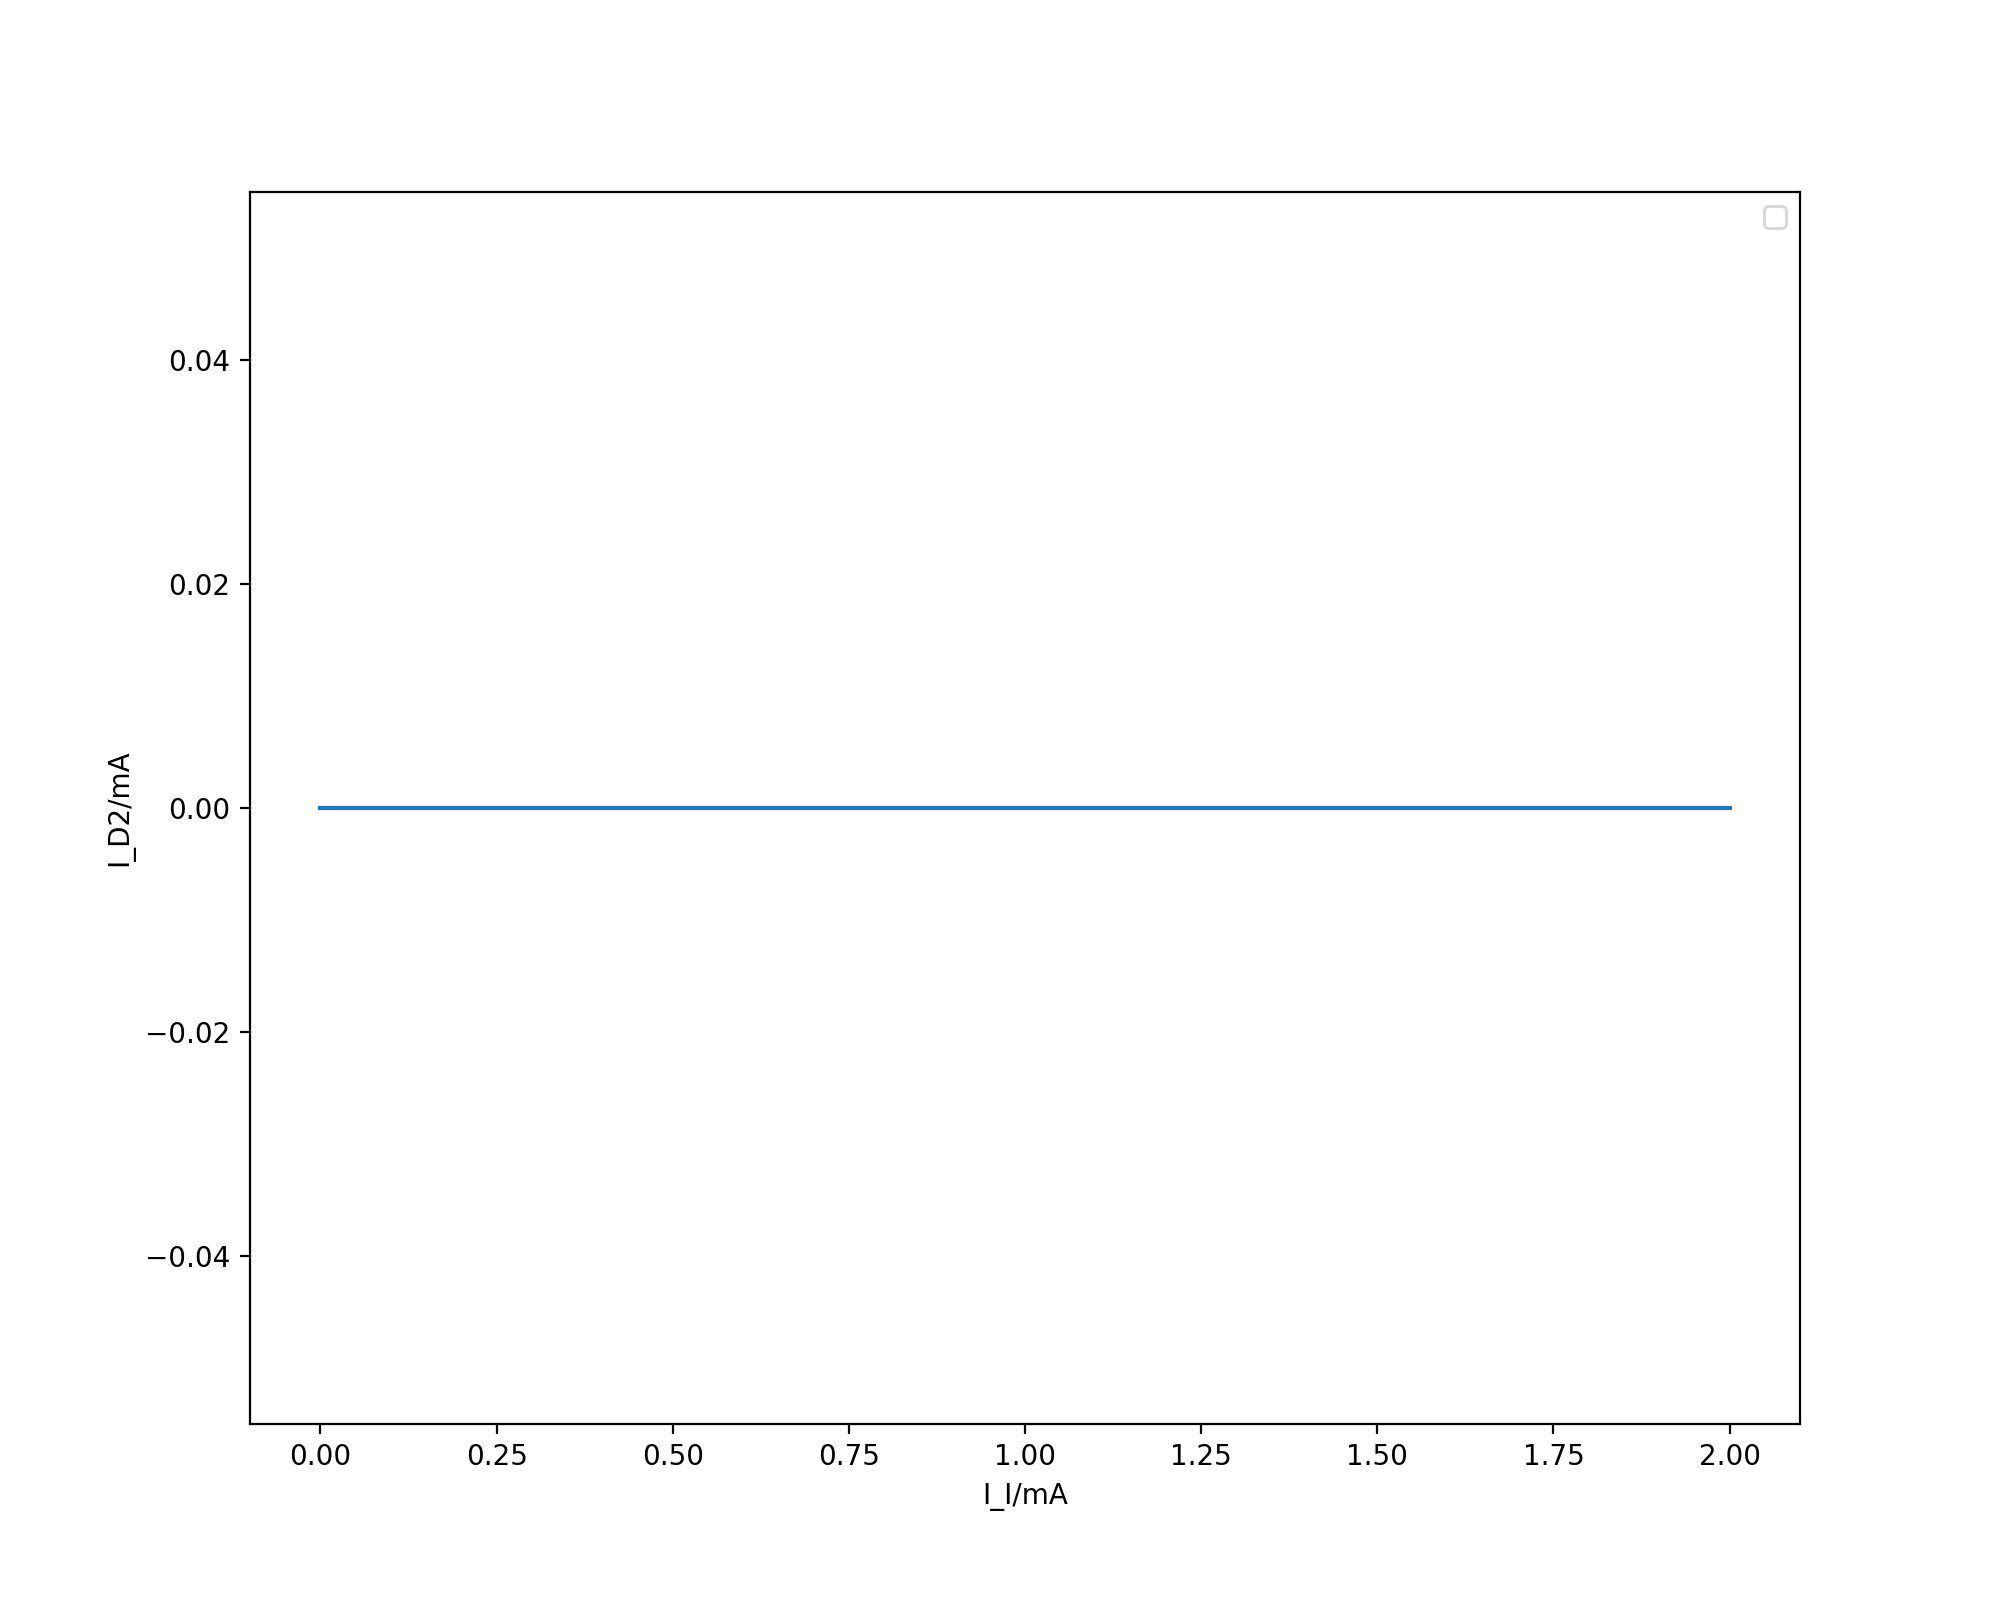
\includegraphics[scale=0.28]{MD1.45_7.png}}
	\caption{(a)}
\end{figure}
\noindent1.50 Assume each diode in the circuit shown in Figure P1.50 has a cut-in voltage
of $V_\gamma = 0.65$V. (a) The input voltage is $V_I = 5$V. Determine the value of
R1 required such that ID1 is one-half the value of $I_{D2}$. What are the values
of $I_{D1}$ and $I_{D2}$? (b) If $V_I = 8V$ and $R_1 = 2k\Omega$, determine $I_{D1}$ and $I_{D2}$.\\
\begin{figure}[H] 
	\centering 
	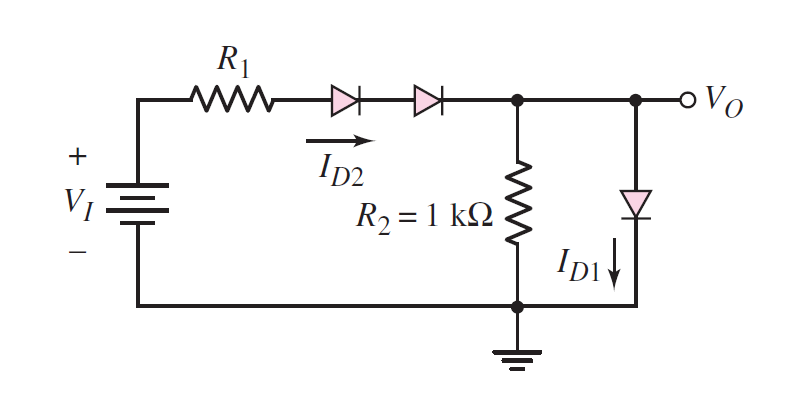
\includegraphics[scale=0.35]{MD1_50.png}
	\caption{Problem 1.50}
\end{figure}
\noindent Solution:\\
(a)Actually, we can know that $D_1$ and $D_2$ are conducted, so we have equation:
$$\begin{cases}
	V_O=V_\gamma\\
	I_{D1}=\displaystyle\frac{1}{2}I_{D2}\\
	V_I-V_O=I_{D2}{R_1}+2V_\gamma\\
	I_{D2}=\displaystyle\frac{V_O}{R_2}+I_{D1}
\end{cases}\Rightarrow
\begin{cases}
	R_1=1.56k\Omega\\
	I_{D2}=1.3\text{mA}\\
	I_{D1}=1.95\text{mA}
\end{cases}
$$
(b)We assume $D_1$ and $D_2$ are conducted, so we have equation
$$\begin{cases}
	V_O=V_\gamma\\
	V_I-V_O=I_{D2}{R_1}+2V_\gamma\\
	I_{D2}=\displaystyle\frac{V_O}{R_2}+I_{D1}
\end{cases}\Rightarrow 
\begin{cases}
	I_{D1}=3.025\text{mA}\\
	I_{D2}=2.375\text{mA}
\end{cases}
$$
\noindent1.57 Consider the Zener diode circuit shown in Figure P1.57. The Zener breakdown
voltage is $V_Z = 5.6$V at $I_Z = 0.1$mA, and the incremental Zener resistance
is $r_z = 10\Omega$. (a) Determine $V_O$ with no load$ (R_L =\infty)$. (b) Find
the change in the output voltage if $V_{PS}$ changes by $\pm1$V. (c) Find $V_O$ if
$V_{PS}$ = 10V and $R_L = 2k\Omega$.\\
\begin{figure}[H] 
	\centering 
	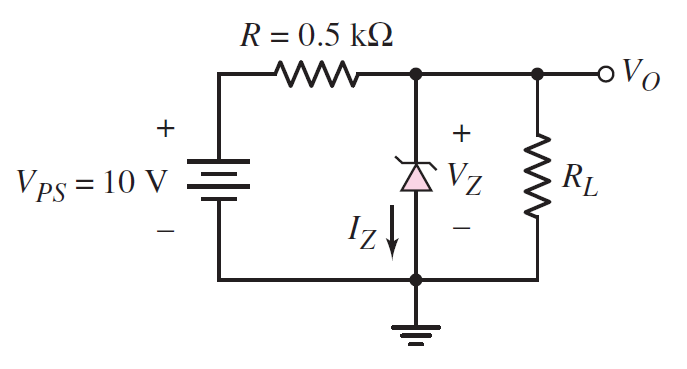
\includegraphics[scale=0.35]{MD1_57.png}
	\caption{Problem 1.57}
\end{figure}
\noindent Solution:\\
(a)Because of KCL and information provided by problem:
$$
	\frac{V_{PS}-V_O}{R}=\frac{V_O-V_z}{r_z}\\
	\Rightarrow V_{O}=5.686\text{V}
$$
(b)When $V_{PS}=9$V:
$$
\frac{V_{PS}-V_O}{R}=\frac{V_O-V_z}{r_z}\\
\Rightarrow V_{O1}=\frac{17}{3}\text{V}
$$
When $V_{PS}=11$V:
$$\begin{aligned}
	&\frac{V_{PS}-V_O}{R}=\frac{V_O-V_z}{r_z}
	\Rightarrow V_{O2}=\frac{97}{17}\text{V}\\
	&\Rightarrow \Delta V_{O}=V_{O1}-V_{O2}=0.0392\text{V}
\end{aligned}	
$$
(c)Because of KCL and information provided by problem, we have equation:
$$
	\frac{V_{PS}-V_O}{R}=\frac{V_O-V_Z}{r_z}+\frac{V_O}{R_L}\\
	\Rightarrow V_O = 5.659 \text{V}
$$
\end{document}